
% --------------------------------------------------------------------------------------
%                   LATEX TEMPLATE FOR DISSERTATION (HONS)
% --------------------------------------------------------------------------------------
\documentclass[11pt]{book}

\usepackage{amsfonts, amsmath, amssymb}  
\usepackage{times}
\usepackage{algorithm}
\usepackage{algorithmic}

%\usepackage[backref=page,pagebackref=true,linkcolor = blue,citecolor = red]{hyperref}
%\usepackage[backref=page]{backref}


\usepackage{graphicx}
\usepackage{listings}
\usepackage{color}

\definecolor{dkgreen}{rgb}{0,0.6,0}
\definecolor{gray}{rgb}{0.5,0.5,0.5}
\definecolor{mauve}{rgb}{0.58,0,0.82}

\lstset{frame=tb,
  language=Java,
  aboveskip=3mm,
  belowskip=3mm,
  showstringspaces=false,
  columns=flexible,
  basicstyle={\small\ttfamily},
  numbers=none,
  numberstyle=\tiny\color{gray},
  keywordstyle=\color{blue},
  commentstyle=\color{dkgreen},
  stringstyle=\color{mauve},
  breaklines=true,
  breakatwhitespace=true,
  tabsize=3
}
\DeclareGraphicsExtensions{.pdf,.png,.jpg}


\setlength{\oddsidemargin}{1.5cm}
\setlength{\evensidemargin}{0cm}
\setlength{\topmargin}{1mm}
\setlength{\headheight}{1.36cm}
\setlength{\headsep}{1.00cm}
%\setlength{\textheight}{20.84cm}
\setlength{\textheight}{19cm}
\setlength{\textwidth}{14.5cm}
\setlength{\marginparsep}{1mm}
\setlength{\marginparwidth}{3cm}
\setlength{\footskip}{2.36cm}



\begin{document}
\pagestyle{empty}

%: ----------------------------------------------------------------------
%:                  TITLE PAGE: name, degree,..
% ----------------------------------------------------------------------


\begin{center}

\vspace{1cm}

%%% Type the thesis title below%%%%%%%%%%%%%%%%
{\Huge         Nested sampling with peers}

\vspace{35mm} 


\includegraphics[width=2cm]{logo}

 \vspace{45mm}

%%%%%Type Your Name Below%%%%%%%%%%%%
{\Large       Feishuang Wang}

	\vspace{1ex}

School of Computer Science

The University of Auckland

	\vspace{5ex}

 %%%%%Typing Your Supervisors Name Below%%%%%%%%%%%%
Supervisor:             Dr Brendon James Brewer

	\vspace{30mm}

A dissertation  submitted in partial fulfillment of the requirements for the degree of Master of Professional Studies in Data Science OR Master of Data Science (delete one), The University of Auckland, 20XX.

\end{center}


  \newpage



%: --------------------------------------------------------------
%:                  FRONT MATTER:  abstract,..
% --------------------------------------------------------------
\chapter*{Abstract}       
\setcounter{page}{1}
\pagestyle{headings}
% \pagenumbering{roman}

\addcontentsline{toc}{chapter}{Abstract}
A nested sampling algorithm is a Bayesian approach to computing and comparing models and generating samples from posterior distributions. We introduce a general Monte Carlo method based on Nested Sampling, which name is Nested Sampling with peers, this method generates one particle above the threshold from the last iteration by querying the params from the server and updating it. We describe the new method over a test case and find that it has better accuracy than the original MCMC-based nested sampling with the same computational overhead.
 Put your abstract  here.  
 The abstract should contain a brief summary of the aim, methodologies, 
finding and conclusions of the dissertation.  The abstract should normally be fewer than 350 words.



%: --------------------------------------------------------------
%:                  END:  abstract
% --------------------------------------------------------------


%: ----------------------- contents ------------------------
\setcounter{secnumdepth}{3} % organisational level that receives a numbers
\setcounter{tocdepth}{3}    % print table of contents for level 3
\tableofcontents            % print the table of contents
% levels are: 0 - chapter, 1 - section, 2 - subsection, 3 - subsection



%: --------------------------------------------------------------
%:                  MAIN DOCUMENT SECTION
% --------------------------------------------------------------
	
\chapter{Introduction}%    \chapter{}  = level 1, top level

\section{Bayesian Analysis} 
The Bayesian Analysis problem is in fact a parameter estimation problem, 
The term \textit{parameter} means \textit{unknown quantity}, howerver in real world, we don't 
have enough information to decide a quantity, so we need Bayesian Analysis to help us.
The parameter you interested in are denoted by $\theta$, to estimate them, first of all, you need to 
model a probability distribution on the \textit{hypothesis space}, a \textit{hypothesis space} is the 
collection of possibilities, this means that you are modeling the initial assumptions, and the probability distribution
is called the \textit{prior}, it is the distribution of $\theta$. The data set is called D, 
after that we can use Bayes’ Theorem to determine the \textit{posterior distribution}:
\begin{equation}
	p(\theta|D) = \frac{p{(\theta)}p(D|\theta)}{p(D)}
\end{equation}
in the above equation, 
\begin{enumerate}
\item The posterior distribution is $p(\theta|D)$, given the data set $D$ with the conditional distribution of $\theta$.
 \item The prior distribution is $p{(\theta)}$.
 \item The likelihood is $p(D|\theta)$, it means the conditional probability of observing the data.
 \item  The denominator $p(D)$ is called marginal likelihood or evidence, it doesn't depend on the parameter $\theta$.
\end{enumerate}
 The posterior distribution is usually more constricted than the prior distribution, 
 indicating that we have gained some insights from the data and that our level of uncertainty about the parameter values has been lowered.
 See the Figure 1.1 for how we often see the updating from the prior distribution to a posterior distribution.
\subsection{Marginal Likelihood}
The marginal likelihood shows how does the model be constructed.
From probability theory we can learn that If you integrate over the posterior distribution, you must get 1 at the last. 
So we can write the marginal likelihood in the following form:
\begin{equation}
	p(D|I) = \int p(\theta|I)p(D|\theta, I)d\theta
\end{equation}
where $I$ represents the underlying assumptions and information, and the integral is N-dimensional, go through all the continuous parameter space, the $I$ is 
usually ignored and the marginal likelihood can be denoted as $Z$:
\begin{equation}
	Z = \int p(\theta)p(D|\theta)d\theta
\end{equation}
when sum the discrete parameter $\theta$, it also has the following form:
\begin{equation}
	Z = \sum p(\theta)p(D|\theta)
\end{equation}
The ratio of evidence values is always called Bayes factors, calculating the value of $Z$ 
is important for comparing different model assumptions, so the Z-value allows the results to be predicted into the future 
because the predicted model can be compared with the current model without the need for recalculation, in short, this parameter measures how well a model fits the data.
However, the standard algorithm such as Markov chain Monte Carlo (MCMC) are considered for posterior distribution, it cannot provide the evidence like Bayesian Inference,
for it only gives a collection of normalised posterior, it will be a challenge to get the evidence in Bayesian analysis.

% The main strength of LaTex is  mathematical typesetting.  

% There is a huge amount of information about LaTex on the internet.
% A helpful short manual, also included in this folder, is the file
% \verb+latex_intro.pdf+
% This document gives a lot of sample LaTex commands.  
% The file \verb+latex-howto.tex+ in this folder also contains examples of many latex commands.
\section{Nested Sampling} 

\subsection{Model Selection with Nested Sampling}
Consider two mutually exclusive model $M_1$ and $M_2$, $M_1$ has the parameter $\theta_1$ and $M_2$ has the 
parameter $\theta_2$, from previous method we discussed, we can calculate the posterior distribution of $\theta_1$ :
\begin{equation}
	p(\theta_1|D, M_1) = \frac{p(\theta_1|M_1)p(D|\theta_1, M_1)}{p(D|M_1)}
\end{equation}
Same, calculate the posterior distribution of $\theta_2$ 
\begin{equation}
	p(\theta_2|D, M_2) = \frac{p(\theta_2|M_2)p(D|\theta_2, M_2)}{p(D|M_2)}
\end{equation}
For simplicity, we often calculate the ratio of posterior distributions to compare models:
\begin{equation}
	\frac{p(M_1|D)}{p(M_2|D)} = \frac{p(M_1)}{p(M_2)} \times \frac{p(D|M_1)}{p(D|M_2)}
\end{equation}
The result of this formula is called \textit{posterior odds}, the posterior probability of M2 over M1 depends on the prior probability: is M2 more credible than M1 before considering the data? Another ratio is the ratio of likelihoods, sometimes called the Bayesian coefficient; how likely is the data for hypothetical M2 versus hypothetical M1? These possibilities are not the likelihood of a particular value of the parameter, but the likelihood of the entire model.
We have to use the marginal likelihood to make a better progress.
\subsection{Sorting}
In multiple dimensions, the direct integration calculation for the edge likelihood becomes unrealistic, we define the 
 $X$ as the model's prior mass, it can be integrated in this form:
 \begin{equation}
	X(\lambda) = \int _{L(\theta)> \lambda}\pi(\theta)d\theta
 \end{equation}
 we can write the inverse function $L(X)$, the marginal likelihood \textit{i.e.} evidence will
 be in this form:
 \begin{equation}
	 Z = \int ^{1}_{0} L(X) dX
 \end{equation}
 To get the inverse function, we can divide the prior into little particles and then sort all the particles by likelihood.
 In geometrical terms, the function $L(X)$ is monotonically diminishing, and the likelihood decreases as the value of X increases from 0 to 1, as shown in Figure 1.1.
From the figure~\ref{fig:modes} we can find that when approaching the maximum likelihood, $X$ will keep decreasing.
 \begin{center}
	\begin{figure}
			\centering
			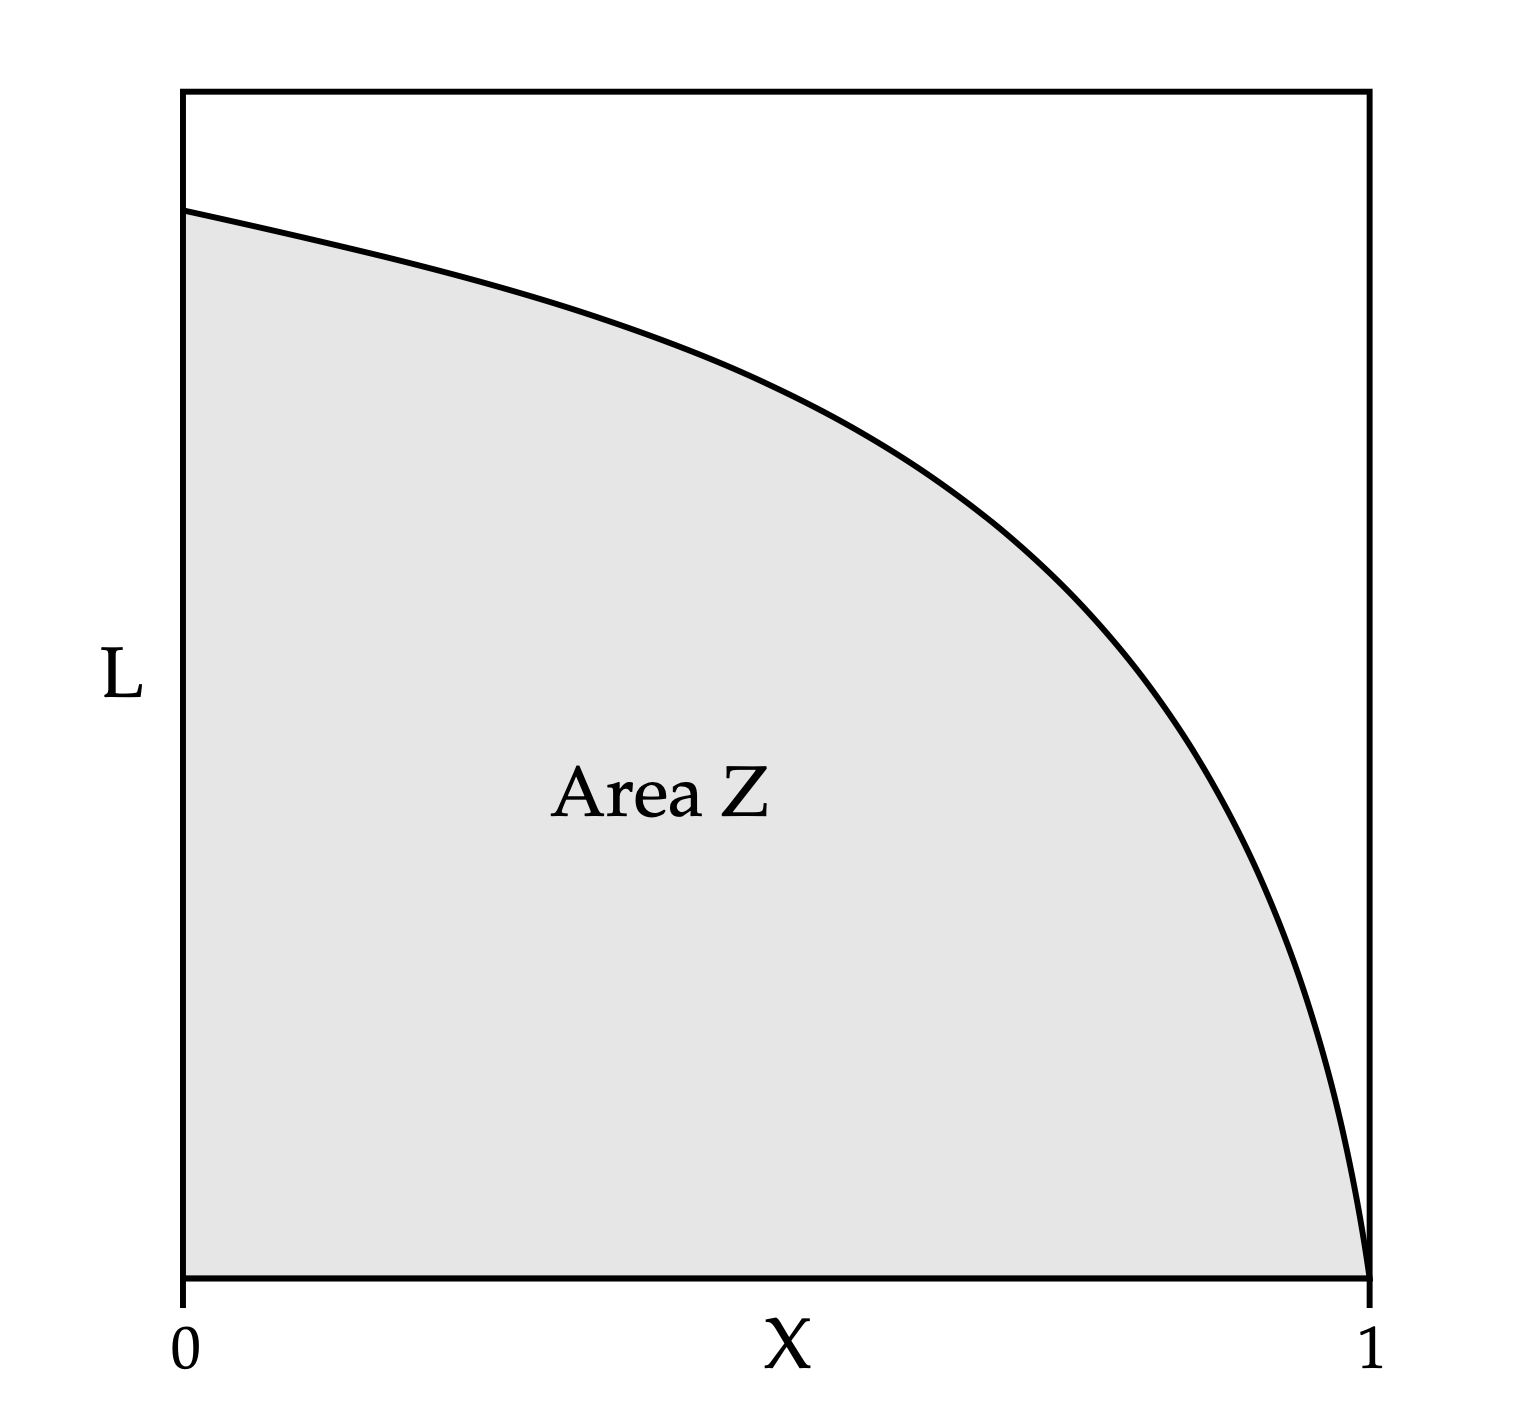
\includegraphics[width=0.6\textwidth]{areaz}
			\caption{Likelihood function with area Z.}
			\label{fig:modes}
	\end{figure}
	\end{center}

The explanation of 1.5 is that the $L(X)$ is the probability corresponding to $\lambda$ that makes the probability, $L(\theta)$, greater than $\lambda$ for $X$. 
$L(0.4) = 0.01$ may be interpreted as a 40$\%$ probability that $\pi(\theta)$ will be greater than 0.01 for $\theta$ chosen from the prior.
To evaluate the mapped integral in 1.5, Skilling proposed a simple trapezoidal rule by calculating 
weighted sums:
\begin{equation}
	Z \approx \sum_{i=1}^{j}w_iL_i (w_i = \frac{1}{2}(X_{i-1} -X_{i+1}))
\end{equation}
In every iteration i, the likelihood is $L(X_i)$, and $j$ is total number of iterations.
\\
---------------------- YOU READ HERE LAST TIME ------------------------------ \\
\\
\\
-------------------------- HERE IS NEW ------------------------------ \\
\\
\subsection{A easy example}
Imagine we have a model whose parameter is a single $X$, and it the parameter $X$ follows the uniform prior distribution
$\pi(\theta)$ from 0 to 1, it also has a likelihood function $L(X)$ which is a decreasing function of X, the Figure~\ref{fig:example1}. illustrate the graph of the example,It's easy to find that in this situation, 
the evidence will be $Z = \int ^ 1 _0L(X)DX$
\begin{center}
	\begin{figure}
			\centering
			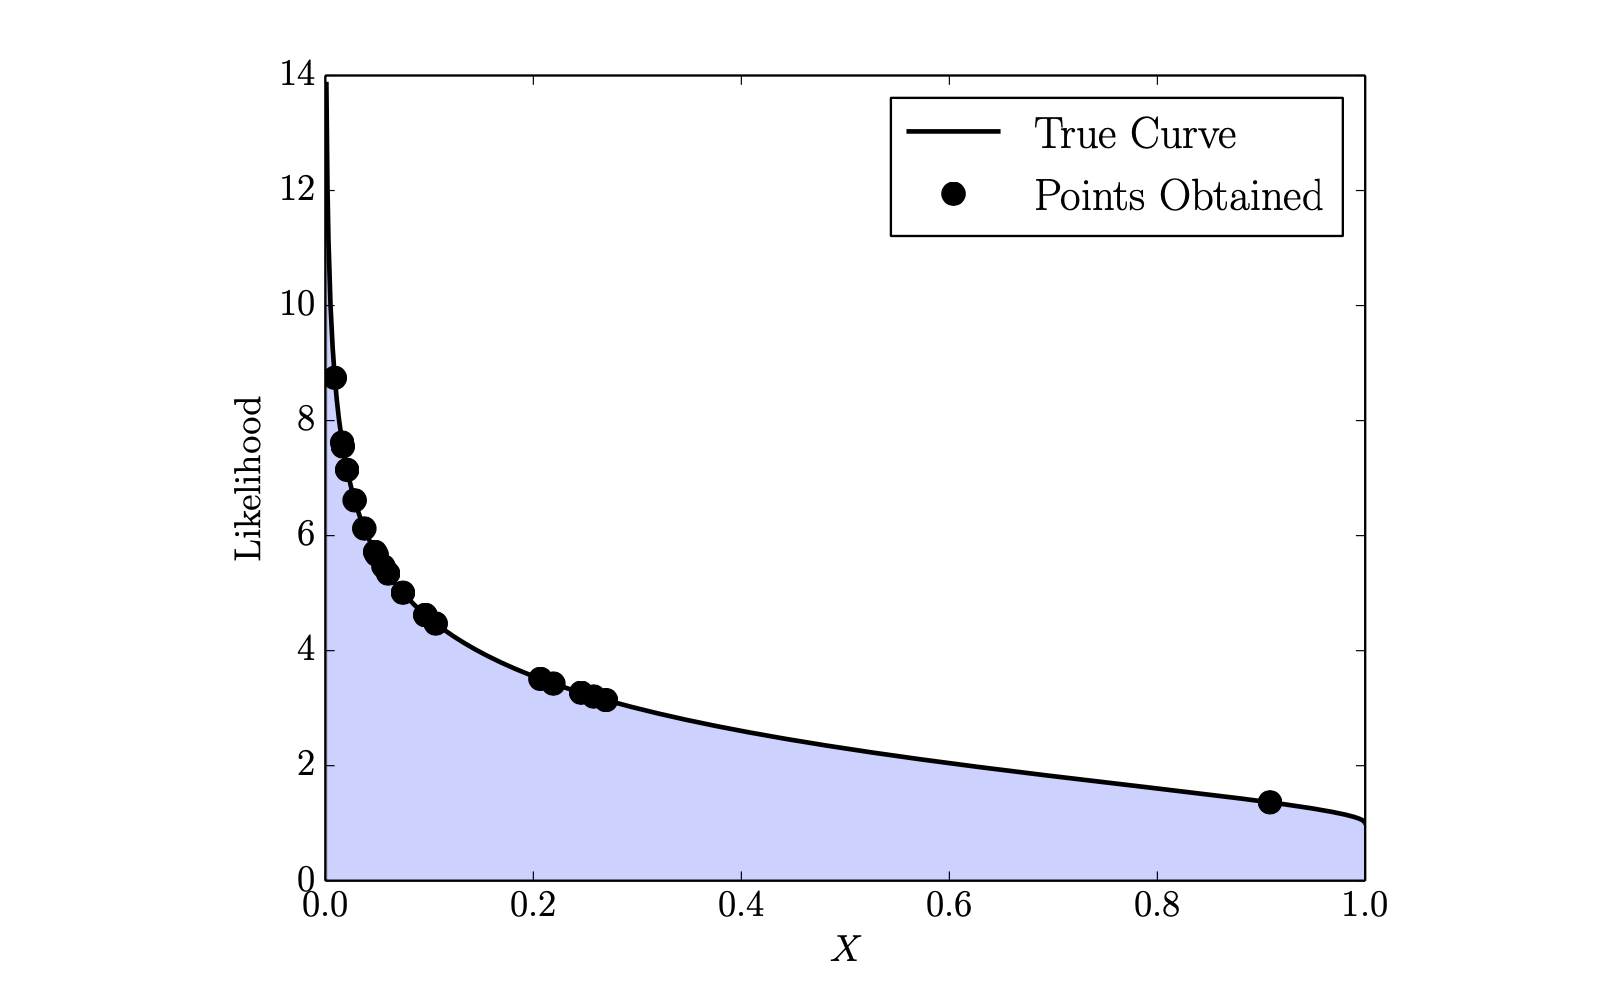
\includegraphics[width=0.6\textwidth]{example1}
			\caption{A simple model estimate problem with only one parameter}
			\label{fig:example1}
	\end{figure}
	\end{center}
\subsection{Nested Sampling Algorithms}
This section will discuss the main idea of Nested Sampling, it is a Monte Carlo algorithm and not a 
typical MCMC algorithm in technical. John Skilling proposed the algorithm specifically for approximating these marginal integrals, \textit{i.e.}, evidence, and it also generates samples from the posterior distribution. 
In the prior distribution $\pi(\theta)$, it needs to generate $N$ \textit{particles or live points} $\theta$, just like an vector to initialize the starting state.
To approximating the evidence, there's some important steps, if we find the points with the worst likelihood,
always denoted by $L_{worst}$ and this is often associated with the highest $X$ value, If different particle $N$ are taken, 
the highest $X$ value will always be close to $X = 1$ and not close to $X = 0$. 
Skilling (2006) gives a simple treatment by estimating $X_{worst} = e^{(\frac{-1}{N})}$, 
and we also know the probability of this point.

By generating a new point $X_1$ from 
the prior distribution $\pi(\theta)$ to replace the worst $X_{worst}$, more points can be obtained,

and the restriction is that the likelihood of the point must be higher than $L_{worst}$.
Also, the prior distribution $\pi(\theta)$ is sampled from the conditional prior, $\pi(\theta | L(\theta > \lambda_{min, 1}))$,
we can denote the new set of particles as $\omega_1=\{\theta|L(\theta> \lambda_{min, 1})\}$, it's a subset of the whole parameter space $\omega$.
And in the second iteration, the estimation of the X value who has a worst particle is $e^{(\frac{-1}{N})} \times e^{(\frac{-1}{N})} = e^{(\frac{-2}{N})}$,
because we already know the likelihood, so we can contiune the iteration.
So the second step to generate the new point $X_2$ and the $X_{worst}$, $X$ will be repeated, we use 
$\omega_2$ to denote them, and we should know that 
$\omega_1 \subset \omega_2$, so the $X_{worst}$ will be replaced, too, from 
the prior distribution $\pi(\theta)$ from the conditional prior, $\pi(\theta | L(\theta > \lambda_{min, 2}))$, so we can write 
when the iteration run $i$ times and it will generate a sequence of $\lambda _{min,i}$ will be like following:
\begin{equation*}
	\lambda _{min,1} < \lambda _{min,2} <  ... < \lambda _{min,i-1} < \lambda _{min,i}
\end{equation*}
,because every $\omega_i$ is subset of the whole space $\omega$, so it will 
decrease continuously, so it can be viewd as as a reduction or compressing
 of the parameter space $\omega$ and the subspaces are nested within each other, 
so we have the term \textit{nested sampling}.
The points $i$ discarded within each loop 
can be sampled using the MCMC algorithm by finding a random copy of a particle
as the initial value , proposed by Skilling (2006). Nowadays, there are also studies 
to investigate whether this approximation can be satisfied
efficiency requirements of MCMC based on 
the shape of the likelihood function and
 the MCMC chosen to explore the restricted prior distribution. (Syarafana Abdul Rahman)

 To estimate the evidence $Z$ we can use the equation give in 1.10, and changing 
 the $w_i = \frac{1}{2}(X_{i-1} -X_{i+1})$ into $\lambda _{min,i}$, which means that the $Z$ can be
 estimate like this:
 \begin{equation}
	\hat{Z} \approx \sum_{i=1}^{j}w_iL_i (w_i = \frac{1}{2}(X_{i-1} -X_{i+1})) = \sum_{i=1}^{j}w_i\lambda _{min,i}
 \end{equation}
 The value of $Z$ will be updated each time based on the results of 
 this approximation until the algorithm terminates according to
  some termination criterion.
\subsection{Prior Mass, X}
Skilling(2006) proposed a method that can decide the prior mass $X$ statistically:
start from $X_0 = 1$, and at each step $i$, a new point $X_i$ is drawn randomly from the prior, 
and the $X_i$ has the restriction that $X_i < X_{i-1}$, this will generate $N$ \textit{live points} that follows the 
 \textit{Uniform(0, $X_{i-1}$)}. The $X$ can be generated like this:
 \begin{equation}
	 X_0 = 1, X_i = t_iX_{i-1}
 \end{equation}
 The $t_i$ is from the $Beta$ distribution where $Beta(N, 1)$, 
 it's the Beta shrinkage, which lowers estimation errors,
 and $t_i = \frac{X_i}{X_{i-1}}, where \;  t_i \in [0,1]$. 
 The recurrence is:
 \begin{equation}
	P(t_i) = Nt^{N-1}_i
 \end{equation}, and it has the expectation that $E(log(t_i)) = -\frac{1}{N}$, 
 and also has the variance that $Var(log(t_i)) = \frac{1}{N^2}$, after $i$ iterations, 
 and the $log^t$ are independent, a rough approximation for the prior mass is $log(x_i) = \sum_{j}^{i=1}log(t_i)$, (Skilling, 2006), 
 and there's another estimation is  $log(x_i) \in [\frac{-(i-\sqrt{i})}{N}, \frac{-(i+\sqrt{i})}{N}]$, proposed by (Sivia and Skilling, 2006),
 this means that The reduction of the prior mass 
 will be linear along the logarithmic X scale.
\subsection{Measuring}
There's another output of Nested Sampling Algorithm is information, this is to find how much were we learnt from the data can be 
measured by the negative relative entropy(Russel, 2017), also 
Burnham and Anderson had proposed the Kullbeck Liebler divergence (Burnham and Anderson, 2001), denoted by information $H$,
this method measures the discrepancy between two distributions, prior distribution and posterior distribution:
\begin{equation}
	H = \int p(\theta|D)log(\frac{p(\theta|D)}{\pi(\theta)})d\theta
\end{equation}
here $p(\theta|D)$ is the posterior distribution. The $\pi(\theta)$ is the prior distribution,
and it can greatly influence the evidence $Z$, if the size of the region of prior mass was concentrated by posterior distribution.
Skilling (2006) proposed that the region is $e^{-H}$, naively, 
a prior distribution that
overlaps with the likelihood function so that the parameter values are consistent will yield less information. This can estimate the uncertainty of $log(Z) = \sqrt{H/N}$ (Skilling, 2006).
On the other hand, if the prior distribution and the likelihood function are concentrated in different regions, more information will be obtained.
After looking at the data, if the prior greatly changed, more information is obtained from the data (Russel, 2017).
If we use $L(X_i)$ to represents the likelihood $X$ at every iteration $i$, 
the value $H$ will be like this:
\begin{equation}
	H = \sum _i w_iL(X_i)/Z \hspace{0.5em} log(L(X_i)/Z)
\end{equation}
\subsection{Nested sampling procedure}
In the begging, the Nested Sampling Algorithm will
generating $N$ particles $\{\theta_1, \theta_2 ,..., \theta_n\}$ from the prior, also has every likelihood 
$\{L(\theta_1), L(\theta_2) ,..., L(\theta_n)\}$, and the lowest value is denoted by $L_{min, i}$, in every iteration $i$,
there are $j$ steps.

The Nested Sampling Algorithm has the following steps:
\begin{algorithm}
	\caption{A}
	\label{alg:A}
	\begin{algorithmic}
	\STATE {Begin with N particles $\{\theta_1, \theta_2 ,..., \theta_n\}$ from the prior.}
	\STATE {\textbf{initialise} $Z=0, X_0=1,i=0$}
	\REPEAT 
	\STATE {for $i = \{1,2,...,j\}$}
	\STATE { \textbf{Find} the particle with the current lowest likelihood values as $L_{min, i}$.}
	\STATE {\textbf{Crude} estimate the value as $X_i = exp(\frac{-i}{N})$}
	\STATE {\textbf{Set} $w_i = X_{i-1} - X_i$}
	\STATE {\textbf{Save} the propertied $(X_i, L_{min, i})$}
	\STATE {\textbf{Increment} $Z$ by $L_{min, i}w_i$}
	\STATE {\textbf{Generate} a new particle from the prior to replace the point above found with $L(\theta) > L_{min, i}$}
	\STATE {\textbf{Increment} the $Z$ by $N^{-1}(L(\theta_1)+...+L(\theta_N))X_j$}
		\UNTIL{Enough iterations have been performed }
	\end{algorithmic}
	\end{algorithm}
\subsection{Nested Sampling Termination Criterion}
To terminate by default, the algorithm has to set some termination criterion.
The termination criterion will depends on the increment of the evidence, which means that 
sum of the evidence has been found enough.
The current found likelihood will make the evidence more significant and $Z_j$ will times a small fraction $f$:
\begin{equation}
	max(L(\theta _1),L(\theta _2),L(\theta _3),...,L(\theta _N))X_j< fZ_j
\end{equation} 

there's some small fraction $f$.
In the previous section we discuss about information, this can be used as a criterion of termination.The $L_iw_i$ is related to the likelihood $L_i$ and width $w_i$, it will increase faster than 
 the widths $w_i$ decreases, and this leads to more regions. (Skilling, 2006). So In the prior mass, the regions we are interested in is $X \approx e^{-H}$, and $X_i \approx e^{-i/H}$, this means 
 the region from the prior found most of the posterior mass. So Skilling proposed a plausible termination criterion 
 that when the iteration $i$ has exceeded $NH$, which means that the information $H$ times the count of 
 live points $N$,
 and practically the number should be set to $2NH$ (Russel, 2007). There's also a scaling constant to ensure that the 
 nested is appropriate, we have:
 \begin{equation}
  ri > N_rH = \sqrt{r}HN
 \end{equation}
 So in this inequality, we can see that we need at least $\sqrt{r}HN$ samples to substitute (Henderson and Goggans, 2013).  
 However, in most circumstances, the user decide when to stop the iteration, because user knows how much information 
 do they need in the current region.
 \section{Distributed System}
 A distributed system is a computing environment in which various components are decentralized
among multiple computers (or other computing devices) on a network. 
These devices work together and synchronize their efforts to get the job done more efficiently 
than if a single device were responsible for the task.
And a distributed system has two main characteristics:
\begin{itemize}
    \item Autonomous computing elements are collected together, and they are independent. In a distributed system,
    when a computer or node has some crash will not affect other computers in the same system,
	it will not  made known to the other components with which it communicates immediately. 
    \item Running program in the same time are a very normal thing in the computer world, all 
	of us doing things without disturbing others, and when it is needed, we can share our resources together.
	The synchronization of concurrently executing programs for shared resources is also an important and recurring topic.
\end{itemize}

\subsection{Example of a distributed system}
Google is the best example of distributed system, it is a pioneer and leader in the field of web search technology,
and it has a very big and complicated sophisticated distributed system, such as searching service and other applications such as youtube and Google Earth.
To design and build this sophisticated distributed system, google has to put efforts from the following points:
\begin{enumerate}
    \item Underlying infrastructure such as big network rooms and databases,as well as various matching settings such as radiators
	Google has numerous data centers scattered around the world. 
	At least 12 significant Google data center installations are located in the United States. 
	The largest known centers are located in The Dalles, Oregon; Atlanta, Georgia; Reston, Virginia; Lenoir, North Carolina; and Moncks Corner, South Carolina (Wikipedia).
    \item To support hundreds of millions files fast and stable reading, writing and searching 
       google has to optimize the distributed file system in many ways such as writing better programs.
    \item To synchronize the files' reading and writing, it also needs a lock system.
    \item A programming model to supports managing very large parallel and distributed computations on the underlying physical infrastructure.
\end{enumerate}

\subsection{Distributed system models}
There're three type of models that can provide an abstract of distributed system:
\begin{enumerate}
	\item \textit{Physical models} show an aspect of distributed system from hardware, 
	explains their underlying connected network and data systems.
	\item \textit{Architectural models} show an aspect from computational elements, 
	computational elements are a single computer or a collection of computers supported by an appropriate network interconnection.
	\item \textit{Fundamental models} To examine individual aspects of distributed systems, we take an abstract perspective, it includes
	three kinds of models: interaction models, which consider the structure and sequencing of the communication between the elements of the system; 
	failure models, which consider the ways in which a system may fail to operate correctly and security models, which consider how the system is protected against attempts to interfere with its correct operation or to steal its data (George, 2006).

\end{enumerate}
In the individual process environment, most of computers use client-server architecture, it's a very simple 
but very important architecture in the history and also use in today's world, 
the process in this architecture is a role of client or server, in particular, 
client processes communicate with individual server processes in potentially independent hosts to 
ask for the  resources like images, videos they manage.
Also, a server can also be clients and asks for resources from other servers, for example a search is not only 
a server, but also a client, for the reason it have to respond queries from users,
which means clients,  then it needs to run crawlers that act as clients of other web servers.
Responding to user queries can be called server task, and requesting other web servers is the client task,
these two tasks are independent with each other, so they can run concurrently.

The figure~\ref{fig:client-server} shows the architecture of client-server modes.

\begin{center}
\begin{figure}[h]
		\centering
		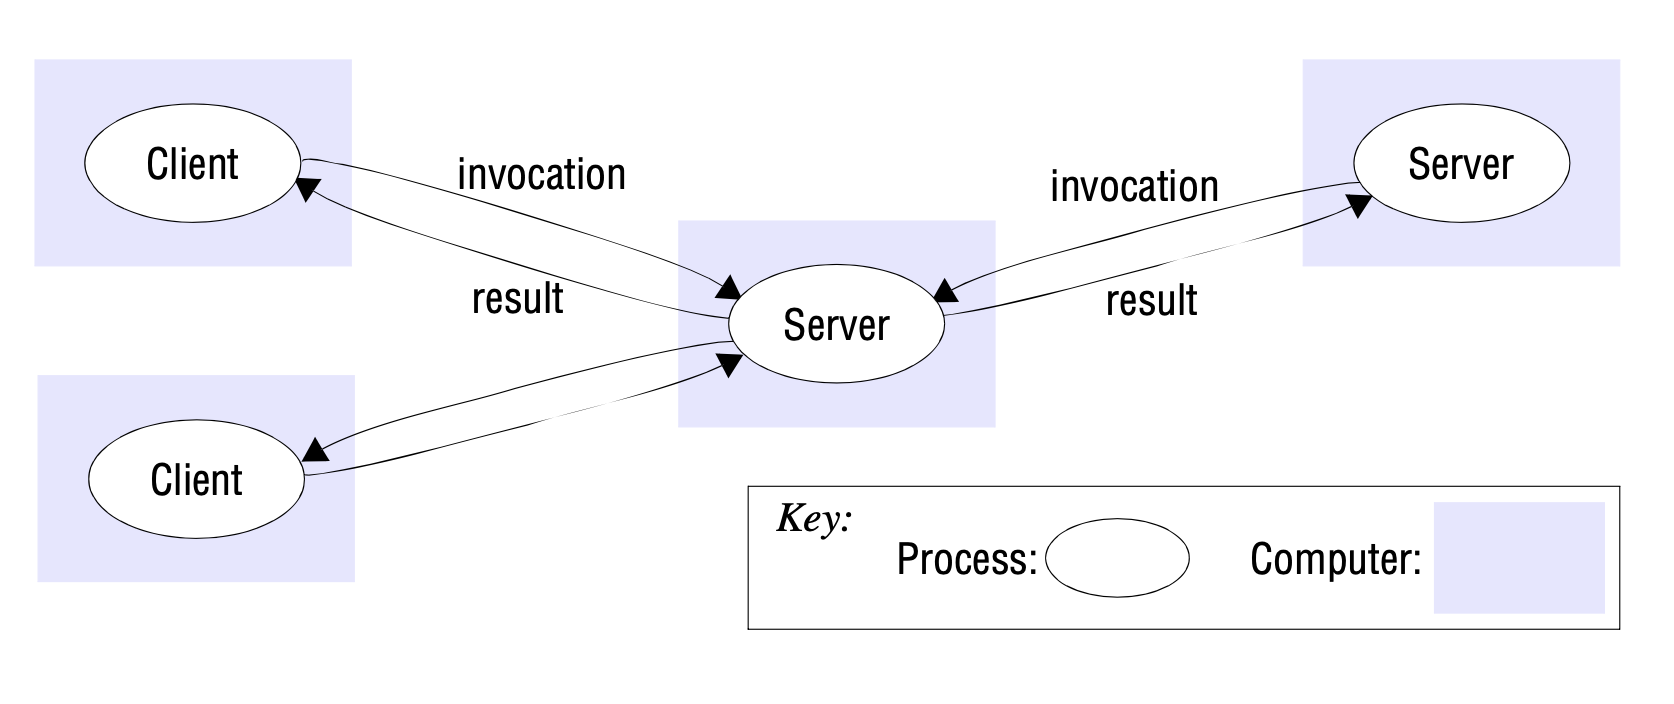
\includegraphics[width=0.6\textwidth]{clien-server}
		\caption{Client-server architecture}
		\label{fig:client-server}
\end{figure}
\end{center}
Although client-server architecture offers a straightforward and relatively simple way to share data 
and manage other resources, it is poorly scalable. 
The server address is relatively single, so it is difficult to expand the computer capacity and network bandwidth.
In the peer-to-peer structure, 
all processes are of the same status and no distinction is made between client and server processes or the computers on which they run. 
In fact, all participating processes run the same programs and provide the same set of APIs to each other.
API stands for  application programming interface, it's a connection between computers 
or between computer processes.
Peer-to-peer architecture can lead to a very useful result that the resources will grow with the number of users. 
This is mainly due to the fact that peer-to-peer was designed with the idea that the network and computing resources owned by the users of a service 
could also be used to support that service.
The figure~\ref{fig:peer-to-peer} shows the architecture of client-server modes.
\begin{center}
	\begin{figure}[h]
			\centering
			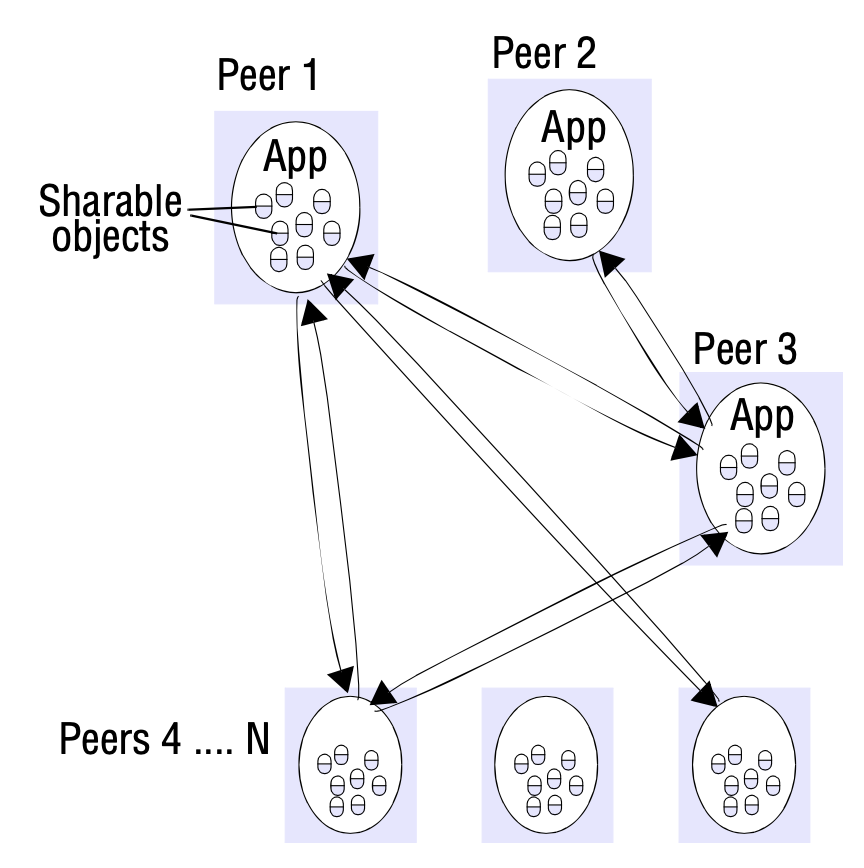
\includegraphics[width=0.6\textwidth]{peer-to-peer}
			\caption{Peer-to-peer architecture}
			\label{fig:peer-to-peer}
	\end{figure}
	\end{center}
	Peer-to-peer architectures can utilize the resources (hardware resources, software resources, data) in almost any computer in the system to accomplish a specific task.
	Here's the advantages of peer-to-peer architecture:
	\begin{enumerate}
		\item 	Better parallel processing capabilities compared to Client-server architecture, 
		which gets slower and slower as more and more clients are added, 
		but p2p networks do not change very much, 
		and all clients can provide resources, 
		including bandwidth, storage space, and computing power.
		\item 	No central server, relying on user groups (peers) to exchange information, 
		reducing network transmission nodes
		\item 	No need to invest a lot of money in server software and hardware.

	\end{enumerate}
	Also, there's some disadvantages of peer-to-peer:
	\begin{enumerate}
		\item More complex architecture, NAT isolation usually exists between nodes and direct communication is not possible, resulting in the need for additional pathway construction process and coordinated management of resources for each node
		\item P2P nodes are spread throughout the Internet, bringing monitoring problems to developers, organizations, and governments
		\item Used in large-scale networks, resource sharing is disorderly and difficult to manage
		\item Lower security
	\end{enumerate}
\subsection{Interprocess communication: sockets}
There are various methods of inter-process communication under unix/linux system, such as
\begin{itemize}
    \item Anonymous pipeline (pipe): communication between parent and child processes
    \item Named pipes (fifo): communication with unrelated processes
    \item Shared memory (shm): can communicate with unrelated processes, need to handle their own process synchronization, such as with semaphore.
	\item Unix domain sockets (unix socket): can communicate with unassociated processes, using the socket interface.
	\item Network socket: can communicate across hosts, using the socket interface.
\end{itemize}
Sockets is one of the most important communication style in distributed system,
A socket is an abstraction of an endpoint for bi-directional communication between application processes on different hosts in a network. A socket is one end of the communication between processes on the network and provides a mechanism for application layer processes to exchange data using network protocols.
e In terms of its position, a socket is connected to the application process and to the network protocol stack, and is the interface through which the application communicates with the network protocol and interacts with the network protocol stack. 
The sockets can be defined as:
\begin{equation}
	sockets = protocol//ip:ports
\end{equation}

The \textit{C++} offers many APIs for socket programming:
\begin{enumerate}
	\item \textbf{socket} Use the function  to create a socket:
		\begin{lstlisting}
			int sockfd = socket(domain, type, protocol)
		\end{lstlisting}
		
 	\item \textbf{bind} function after create the socket, the \textbf{bind} function 
	 binds the socket to the address and port number all together.
	 \begin{lstlisting}
		int bind(int sockfd, const struct sockaddr *addr, 
		socklen_t addrlen);
	 \end{lstlisting}
	 \item \textbf{listen} the server will listen to the ports and waiting for client's connect request.
	 \begin{lstlisting}
		int listen(int sockfd, int backlog);
	 \end{lstlisting}
	 \item \textbf{accept} The textbf{accept} function is called by the TCP server to return the next completed connection from the completed connections queue. If the completed connections queue is empty, then the process is put to sleep (assuming the default blocking mode of socket silence)
	 \begin{lstlisting}
		int listen(int sockfd, int backlog);
		int new_socket= accept(int sockfd, struct sockaddr *addr, socklen_t *addrlen);
	 \end{lstlisting}
	 \item \textbf{connect} The \textbf{connect} function is usually used to establish a tcp connection on the client side.
	 \begin{lstlisting}
		int connect (int sockfd,struct sockaddr * serv_addr,int addrlen);
	 \end{lstlisting}
\end{enumerate}
Here is a basic of network programming procedure using sockets APIs in \textit{C++}:

\begin{lstlisting}
	// server.cpp
    // socket
    int listenfd = socket(AF_INET, SOCK_STREAM, 0);
    // bind
    struct sockaddr_in addr;
    addr.sin_family = AF_INET;
    addr.sin_port = htons(8000);
    addr.sin_addr.s_addr = INADDR_ANY;
    if (bind(listenfd, (struct sockaddr*)&addr, sizeof(addr)) == -1) {
        std::cout << "Error: bind" << std::endl;
        return 0;
    }
    // listen
    if(listen(listenfd, 5) == -1) {
        std::cout << "Error: listen" << std::endl;
        return 0;
    }
    // accept
    int conn;
    char clientIP[INET_ADDRSTRLEN] = "";
    struct sockaddr_in clientAddr;
    socklen_t clientAddrLen = sizeof(clientAddr);
    while (true) {
        conn = accept(listenfd, (struct sockaddr*)&clientAddr, &clientAddrLen);
        inet_ntop(AF_INET, &clientAddr.sin_addr, clientIP, INET_ADDRSTRLEN);

        char buf[255];
        while (true) {
            memset(buf, 0, sizeof(buf));
            int len = recv(conn, buf, sizeof(buf), 0);
            buf[len] = '\0';

            std::cout << buf << std::endl;
            send(conn, buf, len, 0);
        }
        
        close(conn);
    }
    close(listenfd);
    return 0;
	\end{lstlisting}

\begin{lstlisting}
// client.cpp
    // socket
    int client = socket(AF_INET, SOCK_STREAM, 0);

    // connect
    struct sockaddr_in serverAddr;
    serverAddr.sin_family = AF_INET;
    serverAddr.sin_port = htons(8000);
    serverAddr.sin_addr.s_addr = inet_addr("127.0.0.1");
    if (connect(client, (struct sockaddr*)&serverAddr, sizeof(serverAddr)) < 0) {
        std::cout << "Error: connect" << std::endl;
        return 0;
    }
    std::cout << "...connect" << std::endl;
    char data[255];
    char buf[255];
    while (true) {
        send(client, data, strlen(data), 0);
        int len = recv(client, buf, sizeof(buf), 0);
    }
    close(client);
    return 0;
\end{lstlisting}
The figure~\ref{fig:socket} shows diagram of client-server modes in socket programming, which needs many procedure to communicate with 
other computers.
\begin{center}
	\begin{figure}[h]
			\centering
			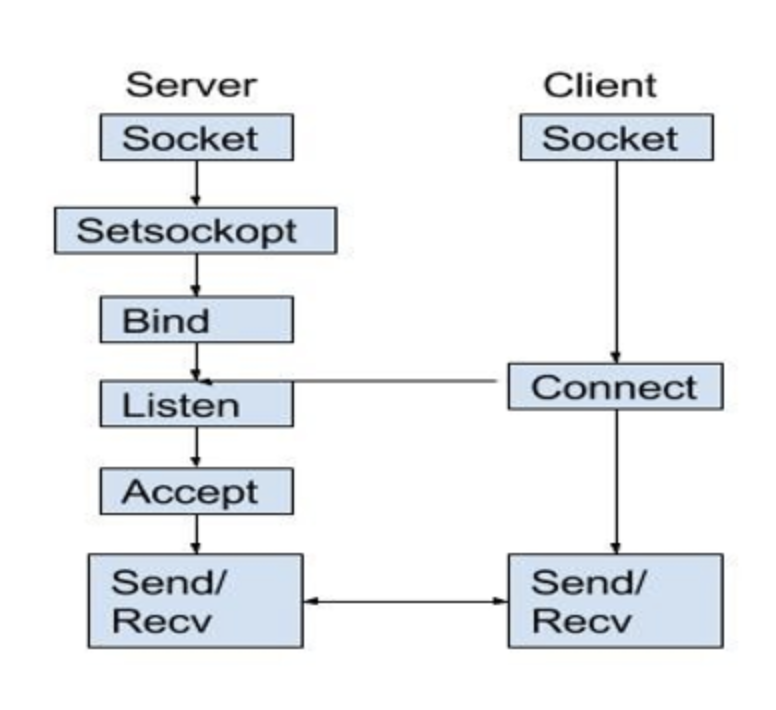
\includegraphics[width=0.6\textwidth]{socket}
			\caption{Socket diagram}
			\label{fig:socket}
	\end{figure}
	\end{center}
\subsection{JavaScript Object Notation: (JSON)}
\textit{JSON} is a text format for data exchange, the current standard is ECMA-404, 
Although JSON is derived from the JavaScript language, it is a data format that can be used in any programming language. There are formats with similar functionality, such as XML and YAML, of which JSON has the simplest syntax.

For example, when a dynamic web page wants to get data from the server, the server looks up the data from the database and converts it into JSON text format:
\begin{lstlisting}
	{
    "title": "Distributed System",
    "subtitle": "How to design better distributed system",
    "author": [
        "Feishuang Wang",
        "Json Jack",
    ],
    "year": 2010,
    "weight": 1.6,
    "hardcover": false,
    "publisher": {
        "Company": "Education",
        "Country": "China"
    },
    "blog": null
}
\end{lstlisting}
The scripting code of the web page can then parse this JSON text into internal data structures for use.

As you can see from this example, JSON is a tree structure, while JSON contains only 6 data types.
\begin{enumerate}
	\item null: it represents by \textbf{null}.
 \item boolean: it represents by \textbf{true} or \textbf{false}.
 \item number: it usually represents by float numbers.
 \item string: it represents by \textbf{`...'}
 \item array: it represents by \textbf{[...]}
 \item object: it represents by \textbf{\{...\}}
\end{enumerate}
JSON parsing fulfills 3 main requirements.
\begin{itemize}
	\item Parse JSON text into a tree data structure (parse).
	\item Provide an interface to access the data structure (access).
 \item Convert the data structure into JSON text (stringify).
\end{itemize}
The figure~\ref{fig:json} the process of parsing a json object:
\begin{center}
	\begin{figure}[h]
			\centering
			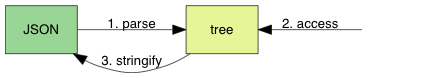
\includegraphics[width=0.6\textwidth]{json}
			\caption{Json parsing}
			\label{fig:json}
	\end{figure}
	\end{center} 
There're many advantages to use json as a format to excahnge data:
\begin{itemize}
	\item Compared with XML, JSON is more concise, we can see the content at a glance, easy to check and troubleshoot.
	\item JSON is lighter, more efficient in writing, transferring, and parsing.
	\item JSON uses compression technology in the transmission process, which saves broadband.
	\item Numerous language support, such as javascript, python, C, C++ and other mainstream languages are supported.
\end{itemize}

\subsection{Berkeley Open Infrastructure for Network Computing: BOINC}
\textit{BOINC} is BOINC is one of the leading distributed computing platforms, 
a decentralized computing system developed by the Department of Computer Science at the University of California, Berkeley. 
Originally designed for the \textit{SETI@home} project, this project is 
SETI stands for Search for Extraterrestrial Intelligence. What this project does is to analyze the data observed by radio telescopes around the world to find three equally spaced convex waves. It is not easy to observe such convex waves because the cosmic waves are very weak and are strongly influenced by the electromagnetic properties of the universe itself.

This kind of task is very suitable for distributed computing, and SETI joined BOINC in the sixth year after the project was established. The nodes that contribute computational power around the world are allowed to join together to find it.
It mainly for research institutions to provide a distributed computing platform. BOINC was developed because many research institutions lack funds, but many research projects require very large computation. So we want to use the distributed computing method to handle large amount of data.
The \textit{BOINC} has many excellent ideas for developers to learn:
\begin{itemize}
	\item Provide dedicated support for the development of advanced algorithms.
 \item Applying artificial intelligence techniques to analyze and process gravitational wave big data, developing more efficient and intelligent algorithms for gravitational wave data analysis, and increasing the possibility of identifying theoretically unknown gravitational waves.
 \item Open up gravitational wave astronomical data and hold challenges to attract companies and citizen scientists to participate and use group intelligence to overcome the problem.
\end{itemize}
\section{Spakslab Problem}
Spike and slab is a more graphic description of a prior.
For a random varible $X$, a spike and slab prior will either gets some value $v$, which can
be called \textit{spike}, or gets some other prior $p_slab(x)$, which will be called \textit{slab}.
The figure~\ref{fig:spike-slab} shows the spike and slab prior:
\begin{center}
	\begin{figure}[h]
			\centering
			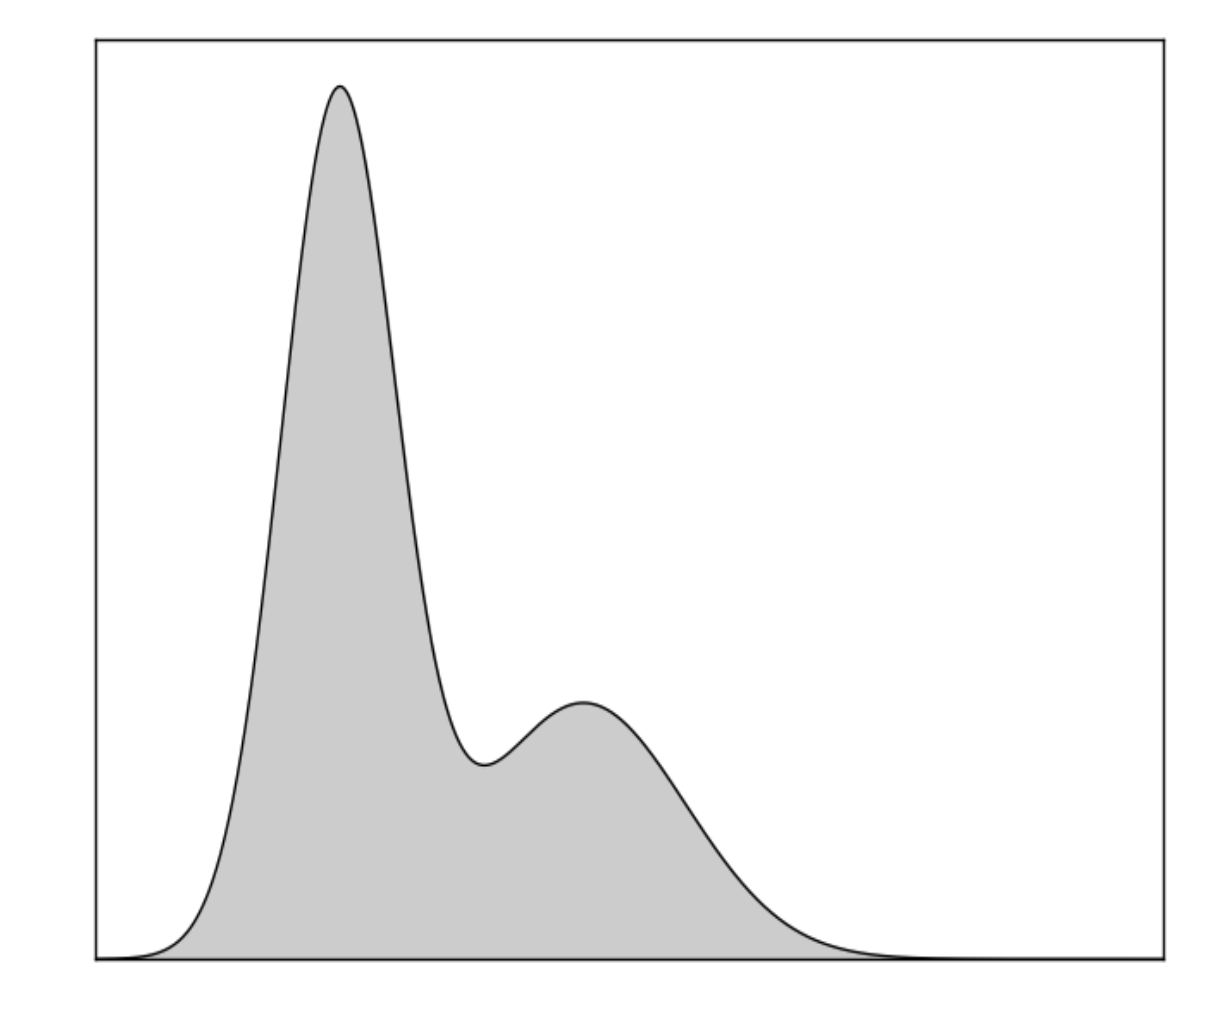
\includegraphics[width=0.6\textwidth]{spike-slab}
			\caption{A view of the spike and slab prior in 2 dimensions. The higher peak is the "spike" and the lower peak is the "slab"}
			\label{fig:spike-slab}
	\end{figure}
	\end{center} 
The spike and slab prior is sparsity inducing in the case that $v=0$ and $X = 0$,
it will give a principled alternative to sparsity-inducing regularisers.
It is used to do Bayesian sparse learning, 
to obtain a sparse model from which further tasks such as feature selection and model compression can be done.
From Bayesian linear regression to Bayesian neural networks, any probabilistic model in a Bayesian framework can be used in spike and slab prior.
The spike and slab correspond to the sampling process that
\begin{enumerate}
	\item For each parameter $w_i$, we first assign a binary indicator $s_i$, which is sampled from a Bernoulli distribution $Bern(p_0)$ and has only two possible values, 0 or 1.
 \item If $s_i=1$, then we continue to draw from a relatively normal and flat Gaussian distribution, such as $N(0,1)$,  at which point the value of $w_i$ has a high probability of not being 0. 
 Conversely, if $s_i=0$ , then we continue to draw from an abnormal and steep Gaussian distribution, such as $N(0,0.000000...1)$ , at which point the value of $w_i$ - is very close to 0.
The probability of the value of $w_i$ is very close to 0, and the effect of sparsity is achieved. 
\end{enumerate}

	
The variance of the spike and slab distribution is $0.000.... .001$, 
but its theoretical value is actually the limit of convergence to 0, 
so it is actually a Dirac delta function $\delta(w_i)$ ($y=1$ except at $x=0$, $y=0$ at other points).
As shown in the figure~\ref{fig:spike-slab-sampling}.
\begin{center}
	\begin{figure}[h]
			\centering
			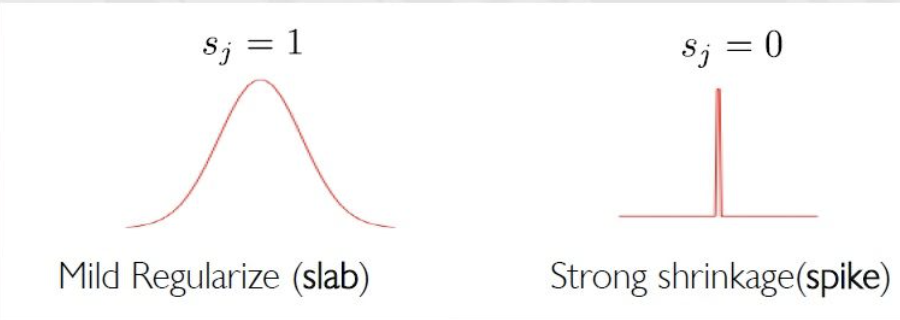
\includegraphics[width=0.6\textwidth]{spike-slab-sampling}
			\caption{A sampling proess of spike and slab.}
			\label{fig:spike-slab-sampling}
	\end{figure}
	\end{center}

	The above steps can be abstracted into the formula:
	\begin{equation}
		P(w_j)=P(s_j)P(w_j|s_j)=Bern(s_j|p_0)(s_jN(w_j|0,\sigma_0^2) + (1-s_j)\delta (w_j))
	\end{equation}
	where $p_0,\sigma_0$ is all hyperparameters. 
	Multiply this in front of your data-likelihood $P(D|W)$ 
	to get a joint distribution of probability models $P(S)P(W|S)P(D|W)$.

	Compared to sparse methods such as L1 loss,
	spike and slab gives a more precise and fine-grained sparse modeling that 
	we can place a unique "sparse prior $p_0$" for each parameter in the model, 
	and also obtain a "sparse probability $c(p_j)$" after extrapolation that describes the probability of each parameter being selected.
	However, some of the most commonly used inference frameworks, such as variational inference and Expectation propogation, cannot be used directly under this kind of prior due to the form of the spike and slab prior (with discontinuous delta functions and mixed Gaussian forms).
	\chapter{Implementation}
\section{The classic nested sampling implementation}
In this section, i implement the classic nested samping algorithm, 
\subsection{Implement the sampler}
\subsection{Sqlite database}


\section{Flask webserver}
\section{Query from the server}
\section{Calculating the MSE}




\begin{enumerate}
\item The basic functions: $\cos(x),  \sin(x),   \ln(x) $,  (\verb+$\cos(x),\sin(x),\ln(x)$+). 
\item Greek letters: $\alpha \beta \gamma \delta\epsilon...$ (\verb+$\alpha\beta\gamma\delta\epsilon...$+).
\item Mathematical symbols: $\int  \oint \sum\lim\bigcup \bigcap$
 (\verb+$\int\oint\sum\lim\bigcup\bigcap$+).
\item Fractions: $\frac{1}{2},\frac{1}{2-x}$ (\verb+$\frac{1}{2},\frac{1}{2-x}$+).
\end{enumerate}

The following matrix 
\begin{eqnarray}\label{eqn:matrix}
\left[
\begin{array}{ccc}
	 U_{r}&     r       &   W_{r}	\\
	   0       &	1      &  V_{x}	\\
	   0	   &	0      &  W_{x}
\end{array}
\right], 
\end{eqnarray}
is generated using  the \verb+equarray+ environment:
\begin{verbatim}
\begin{eqnarray}\label{eqn:matrix}
\left[
\begin{array}{ccc}
	 U_{r}& r &W_{r}\\
	   0 &1 &V_{x}\\
	   0&	0 & W_{x}
\end{array}
\right], 
\end{eqnarray}
\end{verbatim}
The \verb+\label{eqn:matrix}+ command labels the equation with \verb+{eqn:matrix}+ which can 
be referred  to somewhere else in the text by using \verb+\ref{eqn:matrix}+ or  \verb+\eqref{eqn:matrix}+.


The command \verb+\notag+ eliminates the numbering of the first equation,
\begin{eqnarray} \label{eqn:lambda_trace}
\lambda^{(1)}&=&tr[T^{(1)}P],\notag  \\
\lambda^{(2)}&=&tr[T^{(2)}P - T^{(1)}ST^{(1)}P].
\end{eqnarray}
\begin{verbatim}
\begin{eqnarray} \label{eqn:lambda_trace}
\lambda^{(1)}&=&tr[T^{(1)}P],\notag  \\
\lambda^{(2)}&=&tr[T^{(2)}P - T^{(1)}ST^{(1)}P].
\end{eqnarray}
\end{verbatim}


\subsection{Itemized lists}
Example of an itemized list:
\begin{itemize}
\item muscle and fat cells remove glucose from the blood,
\item cells use glucose for protein synthesis.
\end{itemize}
\begin{verbatim}
\begin{itemize}
\item muscle and fat cells remove glucose from the blood,
\item cells use glucose for protein synthesis.
\end{itemize}
\end{verbatim}
This can be done by an enumerated  list:
\begin{enumerate}
\item muscle and fat cells remove glucose from the blood,
\item cells use glucose for protein synthesis.
\end{enumerate}

\begin{verbatim}
\begin{enumerate}
\item muscle and fat cells remove glucose from the blood,
\item cells use glucose for protein synthesis.
\end{enumerate}
\end{verbatim}



\newpage



\subsection{Inserting figures}


You may save your Matlab figures as jpg files.  Figures should  be stored in the 
same folder as the latex files.
For the graphicx package to work you usually need to ask latex to create a pdf file (e.g., command pdflatex or latexpdf).

An example of an inserted image is given in Figure~\ref{fig:modes}.

\begin{center}
\begin{figure}[h]
		\centering
		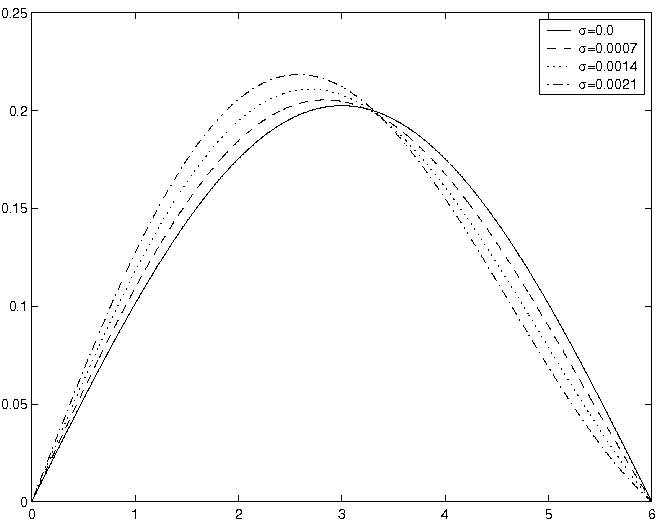
\includegraphics[width=0.6\textwidth]{modes}
		\caption{Mode shapes}
		\label{fig:modes}
\end{figure}
\end{center}




 
\subsection{Tables}\label{table}
Example of a table,
\begin{table}[htp]
\centering
\begin{tabular}{ccc} % ccc means 3 columns, all centered; alternatives are l, r
{\bf Gene} & {\bf GeneID} & {\bf Length} \\ 
\hline % draws a line under the column headers
human latexin & 1234 & 14.9 kbps \\
mouse latexin & 2345 & 10.1 kbps \\
rat latexin   & 3456 & 9.6 kbps \\
\end{tabular}
\caption[title of table]{\textbf{title of table} - Overview of latexin genes.}
\label{latexin_genes} % label for cross-links with \ref{latexin_genes}
\end{table}
\begin{verbatim}
\begin{table}[htp]
\centering
\begin{tabular}{ccc} 
% ccc means 3 columns, all centered; alternatives are l, r
{\bf Gene} & {\bf GeneID} & {\bf Length} \\ 
\hline % draws a line under the column headers
human latexin & 1234 & 14.9 kbps \\
mouse latexin & 2345 & 10.1 kbps \\
rat latexin   & 3456 & 9.6 kbps \\
\end{tabular}
\caption[title of table]{\textbf{title of table} - Overview of latexin genes.}
\label{latexin_genes} % label for cross-links with \ref{latexin_genes}
\end{table}
\end{verbatim}
See how to add two vertical lines in the table (Simply change \verb+{ccc}+ to \verb+{c|c|c}+)
\begin{table}[htp]
\centering
\begin{tabular}{c|c|c} % ccc means 3 columns, all centered; alternatives are l, r
{\bf Gene} & {\bf GeneID} & {\bf Length} \\ 
\hline % draws a line under the column headers
human latexin & 1234 & 14.9 kbps \\
mouse latexin & 2345 & 10.1 kbps \\
rat latexin   & 3456 & 9.6 kbps \\
\end{tabular}
\caption[title of table]{\textbf{title of table} - Overview of latexin genes.}
\label{latexin_genes2} % label for cross-links with \ref{latexin_genes}
\end{table}





\subsection{How to Refer to Equations, Sections, etc}%    \subsection{}    = level 3
 \begin{enumerate}
 \item References can be linked to equations, figures, tables or sections using the command 
 \verb+\ref+:
 Equation (\ref{eqn:lambda_trace}),  Figure~\ref{fig:modes},  Table~\ref{latexin_genes2} and Section~\ref{table}.\\
\verb+Equation~(\ref{eqn:lambda_trace}),Figure~\ref{modes},+\\
\verb+Table~\ref{latexin_genes2} and Section~\ref{table}.+


\item 
Equations can be conveniently  referred to using \verb+ \eqref+. See, for example,  Equation \eqref{eqn:lambda_trace}. \\
\verb+Equation \eqref{eqn:lambda_trace}+\\
Note that \verb+\eqref+ includes the round brackets by itself. 

\item  Citations are in a similar way but using the command \verb+\cite+:

  \cite{Salmond}, \cite{Stull}, and \cite{TandC}, 
   or  \cite{Salmond,Stull,TandC} .
   
  \begin{verbatim}   
   \cite{Salmond}, \cite{Stull}, and \cite{TandC}, 
   or  \cite{Salmond,Stull,TandC} .
 \end{verbatim} 

There are many different styles for writing citations -- you should follow the norms for your subject area.

A more advanced way to do citations is to use \verb+bibtex+.  This is a powerful tool and we encourage you to try it.  There is plenty of information about it on the web.

 
 \end{enumerate}
 
 
 
\chapter{Methodologies and analysis}
\section{Methodologies}
\section{Analysis}
\chapter{Discussion }
\section{Main results}
\section{Discussion}
\chapter{Conclusions}
You may add more chapters as needed in the file.

% --------------------------------------------------------------

% --------------------------------------------------------------
\renewcommand{\bibname}{References} % changes the header; default: Bibliography
\begin{thebibliography}{99} 
\addcontentsline{toc}{chapter}{References}


\bibitem{Farge} Farge Marie, {\em Wavelet Transforms and Their Applications to Turbulence},  \\Ann. Rev. Fluid Mech. volume 24, pages 395-457, 1992.
%ref. for an article
\bibitem{Salmond}  Salmond Jennifer,  {\em Vertical Mixing of Ozone in the Very Stable Nocturnal Boundary Layer}, PhD Thesis, University of British Columbia, 2001.
%ref. for a Thesis.
\bibitem{Stull} Stull B. Ronald, {\em Introduction to Boundary Layer Meteorology}, Dordrecht; Boston: Kulwer Academic Publishers, 1988. %%%ref. for a book
\bibitem{TandC} Torrence Christopher, Compo Gilbert P., {\em A Practical Guide to Wavelet Analysis}, Bulletin of the American Meteorological Society volume 79, pages 61-78, 1998. 
%ref. for an article
\end{thebibliography}


\appendix%%% start appendices here 
\chapter{Some extra things} 

This is an optional chapter for any additional material that does not fit 
conveniently into the body of the text (e.g., data, copies of computer programmes). 
Note that appendices won't necessarily be marked.


\end{document}
